\section{Theorie}
\label{sec:Theorie}
% \begin{equation}
%     \label{eq:}

% \end{equation}
% \begin{figure}[H]
%     \centering
%     \includegraphics[scale=0.5]{content/}
%     \caption{\cite{}.}
%     \label{fig:}
% \end{figure}

%\cite{}
Röntgenstrahlung ist elektromagnetische Strahlung mit Energien oberhalb von $\SI{100}{\electronvolt}$.
Dies entspricht einer Wellenlänge von $\lambda < \SI{1}{\nano\meter}$.

\subsection{Erzeugung von Röntgenstrahlung}
Die Röntgenröhre, in welcher die Röntgenstrahlung erzeugt wird, besteht aus einer evakuierten Röhre, 
in der sich eine Glühkathode und eine Anode befinden.
Der schematische Aufbau ist in Abbildung \ref{fig:roentgenroehre} dargestellt.

\begin{figure}[H]
    \centering
    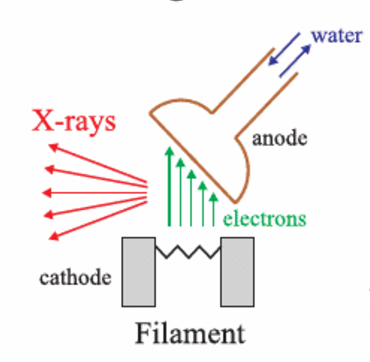
\includegraphics[scale=0.5]{Bilder/tube.png}
    \caption{Schematischer Aufbau einer Röntgenröhre \cite{als-nielsen2011}.}
    \label{fig:roentgenroehre}
\end{figure}

Die Glühkathode emittiert Elektronen durch den glühelektrischen Effekt.
Der glühelektrische Effekt beschreibt die Emission von Elektronen aus einem Festkörper, wenn dieser erhitzt wird.
Die emittierten Elektronen werden durch eine Beschleunigungsspannung $U_\text{B}$ zur Anode hin beschleunigt.
Beim Auftreffen der Elektronen auf die Anode entsteht Röntgenstrahlung \ref{fig:spektrum}.
\begin{figure}[H]
    \centering
    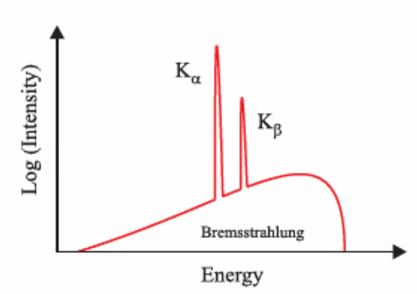
\includegraphics[scale=0.5]{Bilder/spektrum.png}
    \caption{Erzeugte Bremsstrahlung und charakteristische Röntgenstrahlung einer Röntgenröhre \cite{als-nielsen2011}.}
    \label{fig:spektrum}
\end{figure}
Die Röntgenstrahlung setzt sich aus zwei Komponenten zusammen: 
der kontinuierlichen Bremsstrahlung und der charakteristischen Röntgenstrahlung.
Die Bremsstrahlung entsteht, wenn die Elektronen im Coulombfeld der Atomkerne des Anodenmaterials abgebremst werden und dabei Energie verlieren.
Diese Strahlung hat ein kontinuierliches Spektrum, da die Energieabgabe von der Stärke der Abbremsung abhängt.
Die maximale Energie der Bremsstrahlung ist gegeben durch die Beschleunigungsspannung $U_\text{B}$.
Die charakteristische Röntgenstrahlung entsteht, wenn die Elektronen in der Anode in innere Schalen
eines Atoms eindringen und dabei Elektronen aus den Schalen herausschlagen.
Die entstandenen Löcher werden durch Elektronen aus höheren Schalen gefüllt, wobei Röntgenstrahlung emittiert wird.
Die Energie der charakteristischen Röntgenstrahlung ist diskret und entspricht der Energiedifferenz der beteiligten Schalen.
In der Abbildung \ref{fig:spektrum} ist das Spektrum einer Röntgenröhre dargestellt. 
Die $K_\alpha$-Linie entsteht, wenn ein Elektron aus der $L$-Schale in die $K$-Schale fällt, 
während die $K_\beta$-Linie entsteht, wenn ein Elektron aus der $M$-Schale in die $K$-Schale fällt.

\subsection{Röntgenstrahlung an Grenzflächen} \label{sec:reflektivität}
Trifft Röntgenstrahlung auf eine ideal glatte Grenzfläche, 
wie in Abbildung \ref{fig:reflektivität} dargestellt,
gilt für den Brechungsindex $n$ des Mediums
\begin{equation}
    n = 1 - \delta + i\beta,
\end{equation}
wobei $\delta$ und $\beta$ die Dispersion und Absorption des Mediums beschreiben.
\begin{figure}[H]
    \centering
    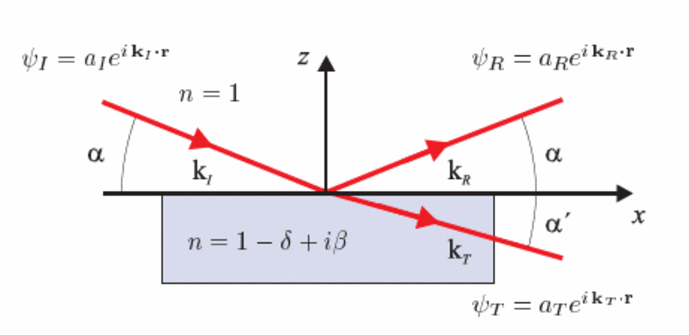
\includegraphics[scale=0.5]{Bilder/reflektion.png}
    \caption{Röntgenstrahlung an einer Grenzfläche \cite{als-nielsen2011}.}
    \label{fig:reflektivität}
\end{figure}
Die Dispersion ist durch die Elektronendichte $\rho$, die Wellenlänge $\lambda$ 
und die Streuamplitude $r_0$ pro Elektron gegeben.
Die Gleichung lautet für die Dispersion lautet
\begin{equation}
    \delta = \frac{r_0 \rho \lambda^2}{2\pi} .
    \label{eq:delta}
\end{equation}
Die Streuamplitude $r_0$ ist gegeben durch die Thomson-Streulänge, 
auch als klassischer Elektronenradius bekannt, und beträgt
\begin{equation}
    r_0 = \SI{2.82e-15}{\meter} .
\end{equation}
Daraus ergibt sich, dass die Dispersion in der Größenordnung von $10^{-6}$ liegt.
Die Absoprtion $\beta$ ist gegeben durch
\begin{equation}
    \beta = \frac{\mu \lambda}{4 \pi} \, ,
    \label{eq:beta}
\end{equation}
wobei $\mu$ der Absorptionskoeffizient ist.